% Drawing 154/07-8 -- folder 154, batch 07, archive page 131 (PDF page 132).
% Transcription: dessins en couleur : plusieurs disques verts ou orange traversés de pseudo-droites orange ; dans deux d'entre eux, un arc vert clair (une pseudo-droite en position relative) et les points d'intersection numérotés sur le bord $1, 2, \ldots, 10$, avec « $11 = 1$ », et dans un troisième, bordé de violet, les points $1, 2, 3, 4$ et $1', 2', 3', 4'$ ; un demi-disque brun au bord orné de petites flèches ; des cercles noirs fléchés ; un rectangle au crayon aux coins numérotés $1, \ldots, 4$ et $1', \ldots, 4'$ ; un cercle au crayon dont le bord porte $\xi_0, \xi_1, \ldots, \xi_{n-2}, \xi_{n-1}$ et $\xi'_1, \xi'_2, \ldots, \xi'_{n-2}$
% Kind: disks with arrangements; arcs in relative position with numbered intersection points; black circles; formulas. Method 2 (schematic redraw from the facsimile). Status: partial.
% Notes: Colour drawings, read from the page view: several green or orange disks crossed by orange pseudolines; in two of them a light green arc (a pseudoline in relative position) and the intersection points numbered on the rim 1, 2, ..., 10, with « 11 = 1 »; in a third, bordered in violet, points numbered with primes; black circles with arrows, empty yellow and pencil circles, a small frame with primed numbers. The numbering is placed evenly along the arcs, not point by point; the pencilled formulas (Circ(I ...), alpha, u^{...}) are text of the transcription. Still differs from the facsimile: see above.
% Coordinates: 1 unit = 1 mm = 1/100 of the crop width (bbox in page fractions: [0.143, 0.098, 0.959, 0.515]).
% Redrawn by Claude (claude-opus-5-5), issue #73, 2026-11-07; not checked by a human; not compiled (no TeX in the session).
% Revised by Claude (claude-opus-5-5) 2026-11-09 (issue #128) after Michel's check: vertices snapped to exact intersections (drawn points on their lines, meeting ends on the stroke they meet, near-concurrent lines through one computed point, curve ends on their rim); labels at \small as in folder 80 batch 3. Status: partial.
% Rights: reproduces part of the work -- behind RENDER_TRANSCRIPTS, never published by itself.
\documentclass[tikz,border=3pt]{standalone}
\usepackage{amsmath,amssymb}
\usetikzlibrary{patterns,arrows.meta}
\tikzset{Or/.style={orange!90!black}, Ye/.style={yellow!80!orange}, Lg/.style={green!60!black!70}, Dg/.style={green!45!black}, Br/.style={brown!80!black}, Rd/.style={red!85!black}, Bl/.style={blue!70!black}, Gy/.style={black!40}, pencil/.style={black!45}, struck/.style={black!35}, mark/.style={circle,draw,inner sep=1.3pt}, pt/.style={circle,fill,inner sep=0.9pt}, opt/.style={circle,draw,fill=white,inner sep=1.1pt}}
\begin{document}
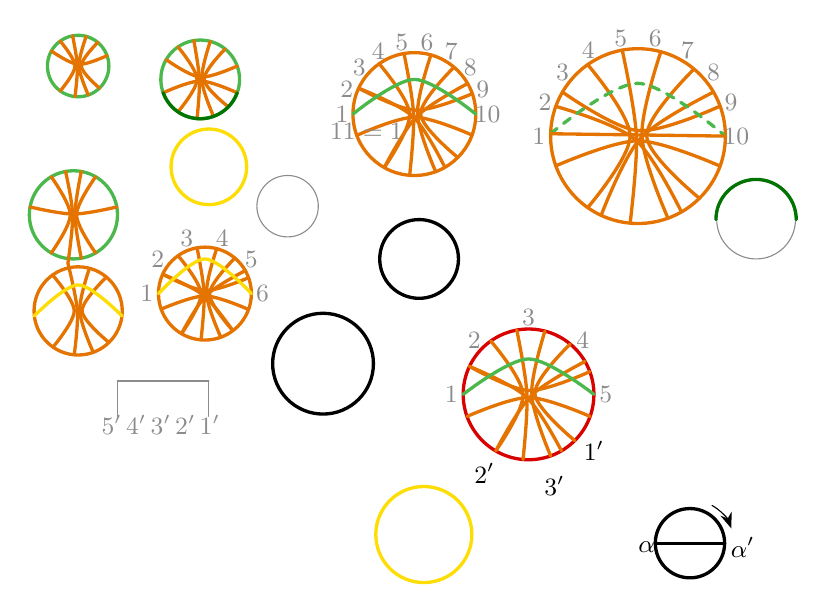
\begin{tikzpicture}[x=1mm,y=1mm,line cap=round,line join=round,font=\scriptsize]
\draw[Lg,very thick] (6.7,-6.1) circle[radius=3.9];
\draw[Or,very thick] plot[smooth, tension=0.55] coordinates {(5.99,-2.26) (6.6,-6.1) (6.3,-9.98)};
\draw[Or,very thick] plot[smooth, tension=0.55] coordinates {(7.72,-2.34) (6.8,-6.1) (7.99,-9.78)};
\draw[Or,very thick] plot[smooth, tension=0.55] coordinates {(4.42,-2.93) (6.3,-6.1) (4.42,-9.27)};
\draw[Or,very thick] plot[smooth, tension=0.55] coordinates {(9.2,-3.1) (7.1,-6.1) (9.41,-8.91)};
\draw[Or,very thick] plot[smooth, tension=0.55] coordinates {(3.3,-4.2) (6.7,-5.9) (10.37,-4.78)};
\draw[Lg,very thick] (22.2,-7.8) circle[radius=5];
\draw[Or,very thick] plot[smooth, tension=0.55] coordinates {(21.39,-2.87) (22.1,-7.8) (21.8,-12.78)};
\draw[Or,very thick] plot[smooth, tension=0.55] coordinates {(23.48,-2.97) (22.4,-7.8) (23.9,-12.5)};
\draw[Or,very thick] plot[smooth, tension=0.55] coordinates {(19.38,-3.67) (21.8,-7.8) (19.38,-11.92)};
\draw[Or,very thick] plot[smooth, tension=0.55] coordinates {(25.37,-3.93) (22.7,-7.8) (25.78,-11.29)};
\draw[Or,very thick] plot[smooth, tension=0.55] coordinates {(17.88,-5.29) (22.2,-7.5) (26.9,-6.1)};
\draw[Or,very thick] plot[smooth, tension=0.55] coordinates {(17.5,-9.5) (22.2,-8) (26.9,-9.5)};
\draw[Lg,very thick] (6.1,-25) circle[radius=5.6];
\draw[Or,very thick] plot[smooth, tension=0.55] coordinates {(5.1,-19.49) (6,-25) (5.4,-31.15)};
\draw[Or,very thick] plot[smooth, tension=0.55] coordinates {(7.1,-19.49) (6.3,-25) (7.1,-30.51)};
\draw[Or,very thick] plot[smooth, tension=0.55] coordinates {(3.28,-20.16) (5.7,-25) (3.28,-29.84)};
\draw[Or,very thick] plot[smooth, tension=0.55] coordinates {(8.92,-20.16) (6.5,-25) (8.92,-29.84)};
\draw[Or,very thick] plot[smooth, tension=0.55] coordinates {(0.59,-24) (6.1,-24.9) (11.61,-24)};
\draw[Or,very thick] (6.7,-37.2) circle[radius=5.6];
\draw[Or,very thick] plot[smooth, tension=0.55] coordinates {(5.4,-31.15) (6.6,-37.2) (6.2,-42.78)};
\draw[Or,very thick] plot[smooth, tension=0.55] coordinates {(8.13,-31.79) (6.9,-37.2) (8.62,-42.46)};
\draw[Or,very thick] plot[smooth, tension=0.55] coordinates {(3.45,-32.64) (6.2,-37.2) (3.5,-41.8)};
\draw[Or,very thick] plot[smooth, tension=0.55] coordinates {(10.29,-32.9) (7.2,-37.2) (10.61,-41.21)};
\draw[Or,very thick] (22.8,-35) circle[radius=5.9];
\draw[Or,very thick] plot[smooth, tension=0.55] coordinates {(21.8,-29.19) (22.7,-35) (22.3,-40.88)};
\draw[Or,very thick] plot[smooth, tension=0.55] coordinates {(24.3,-29.29) (23,-35) (24.82,-40.54)};
\draw[Or,very thick] plot[smooth, tension=0.55] coordinates {(19.39,-30.19) (22.3,-35) (19.85,-40.05)};
\draw[Or,very thick] plot[smooth, tension=0.55] coordinates {(26.61,-30.49) (23.4,-35) (26.3,-39.65)};
\draw[Or,very thick] plot[smooth, tension=0.55] coordinates {(17.45,-32.55) (22.8,-34.6) (28.34,-32.98)};
\draw[Or,very thick] plot[smooth, tension=0.55] coordinates {(17.24,-36.98) (22.8,-35.3) (28.34,-37.02)};
\draw[Or,very thick] plot[smooth, tension=0.55] coordinates {(27.93,-32.08) (23,-35.2) (19.85,-40.05)};
\draw[Or,very thick] plot[smooth, tension=0.55] coordinates {(17.45,-32.55) (22.6,-35.2) (26.3,-39.65)};
\draw[Or,very thick] (49.4,-12.2) circle[radius=7.8];
\draw[Or,very thick] plot[smooth, tension=0.55] coordinates {(48.08,-4.51) (49.3,-12.2) (48.8,-19.98)};
\draw[Or,very thick] plot[smooth, tension=0.55] coordinates {(51.5,-4.69) (49.8,-12.2) (52.11,-19.52)};
\draw[Or,very thick] plot[smooth, tension=0.55] coordinates {(44.93,-5.81) (48.8,-12.2) (45.6,-18.95)};
\draw[Or,very thick] plot[smooth, tension=0.55] coordinates {(54.44,-6.25) (50.2,-12.2) (54.92,-17.72)};
\draw[Or,very thick] plot[smooth, tension=0.55] coordinates {(42.4,-8.95) (49.5,-11.7) (56.76,-9.61)};
\draw[Or,very thick] plot[smooth, tension=0.55] coordinates {(42.08,-14.91) (49.4,-12.6) (56.73,-14.87)};
\draw[Or,very thick] plot[smooth, tension=0.55] coordinates {(56.17,-8.32) (49.7,-12.5) (45.6,-18.95)};
\draw[Or,very thick] plot[smooth, tension=0.55] coordinates {(42.4,-8.95) (49.2,-12.5) (53.28,-18.97)};
\draw[Or,very thick] (77.8,-15) circle[radius=11.1];
\draw[Or,very thick] plot[smooth, tension=0.55] coordinates {(75.8,-4.08) (77.6,-15) (76.8,-26.06)};
\draw[Or,very thick] plot[smooth, tension=0.55] coordinates {(80.7,-4.29) (78.3,-15) (81.61,-25.43)};
\draw[Or,very thick] plot[smooth, tension=0.55] coordinates {(71.41,-5.92) (76.8,-15) (71.41,-24.08)};
\draw[Or,very thick] plot[smooth, tension=0.55] coordinates {(84.92,-6.48) (78.9,-15) (85.6,-22.9)};
\draw[Or,very thick] plot[smooth, tension=0.55] coordinates {(68.21,-9.41) (77.8,-14.3) (88.23,-11.19)};
\draw[Or,very thick] plot[smooth, tension=0.55] coordinates {(67.36,-18.78) (77.8,-15.6) (88.23,-18.81)};
\draw[Or,very thick] plot[smooth, tension=0.55] coordinates {(87.39,-9.41) (78.1,-15.3) (73.12,-25.06)};
\draw[Or,very thick] plot[smooth, tension=0.55] coordinates {(67.36,-11.22) (77.4,-15.4) (83.32,-24.63)};
\draw[Rd,very thick] (63.9,-47.8) circle[radius=8.3];
\draw[Or,very thick] plot[smooth, tension=0.55] coordinates {(62.41,-39.64) (63.7,-47.8) (63.2,-56.07)};
\draw[Or,very thick] plot[smooth, tension=0.55] coordinates {(65.98,-39.77) (64.3,-47.8) (66.7,-55.61)};
\draw[Or,very thick] plot[smooth, tension=0.55] coordinates {(59.11,-41.02) (63.2,-47.8) (59.75,-54.95)};
\draw[Or,very thick] plot[smooth, tension=0.55] coordinates {(69.19,-41.41) (64.7,-47.7) (69.77,-53.67)};
\draw[Or,very thick] plot[smooth, tension=0.55] coordinates {(56.4,-44.25) (63.9,-47.3) (71.68,-44.91)};
\draw[Or,very thick] plot[smooth, tension=0.55] coordinates {(56.09,-50.6) (63.9,-48.2) (71.71,-50.6)};
\draw[Or,very thick] plot[smooth, tension=0.55] coordinates {(71.07,-43.62) (64.2,-48) (59.75,-54.95)};
\draw[Or,very thick] plot[smooth, tension=0.55] coordinates {(56.4,-44.25) (63.6,-48.1) (68.08,-54.97)};
\draw[Dg,very thick] (17.5,-9.5) arc[start angle=200, end angle=340, x radius=5, y radius=5];
\draw[Ye,very thick] (23.3,-18.9) circle[radius=4.8];
\draw[pencil] (33.3,-23.9) circle[radius=3.9];
\draw[Ye,very thick] plot[smooth, tension=0.55] coordinates {(1.14,-37.83) (6.7,-33.9) (12.26,-37.83)};
\draw[Ye,very thick] plot[smooth, tension=0.55] coordinates {(16.9,-35) (22.8,-30.6) (28.7,-35)};
\node[inner sep=1pt,pencil] at (15.4,-35) {\small 1};
\node[inner sep=1pt,pencil] at (16.8,-30.7) {\small 2};
\node[inner sep=1pt,pencil] at (20.5,-28) {\small 3};
\node[inner sep=1pt,pencil] at (25,-28) {\small 4};
\node[inner sep=1pt,pencil] at (28.7,-30.7) {\small 5};
\node[inner sep=1pt,pencil] at (30.1,-35) {\small 6};
\draw[Lg,very thick] plot[smooth, tension=0.55] coordinates {(41.6,-12.2) (49.4,-7.8) (57.2,-12.2)};
\node[inner sep=1pt,pencil] at (40.2,-12.2) {\small 1};
\node[inner sep=1pt,pencil] at (40.8,-9.1) {\small 2};
\node[inner sep=1pt,pencil] at (42.4,-6.3) {\small 3};
\node[inner sep=1pt,pencil] at (44.8,-4.2) {\small 4};
\node[inner sep=1pt,pencil] at (47.8,-3.1) {\small 5};
\node[inner sep=1pt,pencil] at (51,-3.1) {\small 6};
\node[inner sep=1pt,pencil] at (54.1,-4.2) {\small 7};
\node[inner sep=1pt,pencil] at (56.5,-6.3) {\small 8};
\node[inner sep=1pt,pencil] at (58.1,-9.1) {\small 9};
\node[inner sep=1pt,pencil] at (58.7,-12.2) {\small 10};
\node[inner sep=1pt,pencil] at (43.3,-14.4) {\small $11=1$};
\draw[Lg,dashed,very thick] plot[smooth, tension=0.55] coordinates {(66.7,-14.7) (77.8,-8.3) (88.9,-15)};
\node[inner sep=1pt,pencil] at (65.2,-15) {\small 1};
\node[inner sep=1pt,pencil] at (66,-10.7) {\small 2};
\node[inner sep=1pt,pencil] at (68.2,-6.9) {\small 3};
\node[inner sep=1pt,pencil] at (71.5,-4.1) {\small 4};
\node[inner sep=1pt,pencil] at (75.6,-2.6) {\small 5};
\node[inner sep=1pt,pencil] at (80,-2.6) {\small 6};
\node[inner sep=1pt,pencil] at (84.1,-4.1) {\small 7};
\node[inner sep=1pt,pencil] at (87.4,-6.9) {\small 8};
\node[inner sep=1pt,pencil] at (89.6,-10.7) {\small 9};
\node[inner sep=1pt,pencil] at (90.3,-15) {\small 10};
\draw[Or,very thick] (66.7,-14.7) -- (88.9,-15);
\draw[Lg,very thick] plot[smooth, tension=0.55] coordinates {(55.6,-47.8) (63.9,-43.3) (72.2,-47.8)};
\node[inner sep=1pt,pencil] at (54.1,-47.8) {\small 1};
\node[inner sep=1pt,pencil] at (57,-40.9) {\small 2};
\node[inner sep=1pt,pencil] at (63.9,-38) {\small 3};
\node[inner sep=1pt,pencil] at (70.8,-40.9) {\small 4};
\node[inner sep=1pt,pencil] at (73.7,-47.8) {\small 5};
\node[inner sep=1pt] at (58.3,-57.8) {\small $2'$};
\node[inner sep=1pt] at (67.2,-59.4) {\small $3'$};
\node[inner sep=1pt] at (72.2,-55) {\small $1'$};
\draw[pencil] (92.8,-25.6) circle[radius=5];
\draw[Dg,very thick] (97.9,-25.6) arc[start angle=0, end angle=180, x radius=5.1, y radius=5.1];
\draw[very thick] (50,-30.6) circle[radius=5];
\draw[very thick] (37.8,-43.9) circle[radius=6.4];
\draw[Ye,very thick] (50.6,-65.6) circle[radius=6.1];
\draw[very thick] (84.4,-66.7) circle[radius=4.4];
\draw[very thick] (80,-66.7) -- (88.8,-66.7);
\node[inner sep=1pt] at (78.9,-67.2) {\small $\alpha$};
\node[inner sep=1pt] at (91.1,-67.2) {\small $\alpha'$};
\draw[-{Stealth[length=2mm]}] (87.2,-61.9) arc[start angle=60, end angle=20, x radius=5.6, y radius=5.6];
\draw[pencil] (11.7,-46.1) -- (23.3,-46.1);
\draw[pencil] (11.7,-46.1) -- (11.7,-50.6);
\draw[pencil] (23.3,-46.1) -- (23.3,-50.6);
\node[inner sep=1pt,pencil] at (17.2,-51.7) {\small $5'\,4'\,3'\,2'\,1'$};
\end{tikzpicture}
\end{document}
